% ============================================================================
% V. RESULTS (REVISED)
% ============================================================================
\section{Results}
\label{sec:results}
% ----------------------------------------------------------------------------
\subsection{Autoencoder Performance}
\label{sec:results_autoencoder}

The 3D CAE converged reliably across multiple training runs, demonstrating stable representation learning for 4D ME-HSI data.

\subsubsection{Training Convergence}
Figure~\ref{fig:training} shows representative training curves.
The masked MSE loss decreased from approximately 0.45 to 0.03 over 25--30 epochs, with smooth convergence and no evidence of overfitting (training and validation losses tracked closely).
Learning rate reductions triggered at epochs 15 and 22 refined convergence.
Early stopping typically activated between epochs 25--30.

\begin{figure}[!t]
\centering
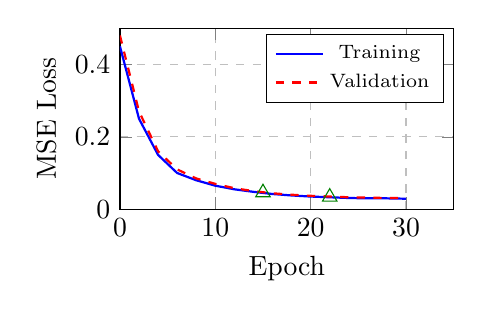
\begin{tikzpicture}
\begin{axis}[
    width=0.48\textwidth,
    height=0.32\textwidth,
    xlabel={Epoch},
    ylabel={MSE Loss},
    xmin=0, xmax=35,
    ymin=0, ymax=0.5,
    grid=major,
    grid style={dashed, gray!50},
    legend pos=north east,
    legend style={font=\scriptsize},
]

% Training loss curve
\addplot[blue, thick] coordinates {
    (0, 0.45) (2, 0.25) (4, 0.15) (6, 0.10) (8, 0.08) (10, 0.065)
    (12, 0.055) (14, 0.048) (16, 0.042) (18, 0.038) (20, 0.035)
    (22, 0.033) (24, 0.031) (26, 0.030) (28, 0.030) (30, 0.029)
};
\addlegendentry{Training}

% Validation loss curve
\addplot[red, thick, dashed] coordinates {
    (0, 0.48) (2, 0.27) (4, 0.16) (6, 0.11) (8, 0.085) (10, 0.070)
    (12, 0.058) (14, 0.050) (16, 0.044) (18, 0.040) (20, 0.037)
    (22, 0.035) (24, 0.033) (26, 0.032) (28, 0.031) (30, 0.031)
};
\addlegendentry{Validation}

% LR reduction markers
\addplot[only marks, mark=triangle, mark size=3pt, green!50!black] coordinates {(15, 0.046) (22, 0.034)};

\end{axis}
\end{tikzpicture}
\caption{Training convergence curves for the 3D CAE. Loss decreased smoothly from 0.45 to 0.03 over 30 epochs. Green triangles indicate learning rate reductions.}
\label{fig:training}
\end{figure}

\subsubsection{Reconstruction Quality}
The trained autoencoder achieved RMSE of 0.078 and PSNR of 22.16\,dB on the validation set.
Visual inspection confirmed that reconstructions preserved key spectral features across all excitation wavelengths.
Per-excitation analysis showed consistent reconstruction quality, with no systematic degradation at particular excitation wavelengths.

\subsubsection{Latent Space Quality}
Analysis of the 20-dimensional latent space revealed meaningful variation.
The top 5 dimensions by variance accounted for 72\% of total latent variance, indicating that information was distributed but concentrated in a subset of dimensions.
This supported using top-$k$ dimension selection for perturbation analysis.

% ----------------------------------------------------------------------------
\subsection{Wavelength Selection Results}
\label{sec:results_selection}

Using all 192 wavelength pairs with KNN classification established a baseline of 88.2\% accuracy ($\kappa = 0.842$).
Per-class performance varied: Class~1 achieved 99.1\% recall and 98.0\% precision, while Classes~2 and~3 showed mutual confusion (15,846 Class~3 pixels misclassified as Class~2), reflecting spectral overlap in their fluorescence signatures.
This confusion pattern persisted across all wavelength selections, indicating a fundamental limitation of the spectral data rather than the selection method.

Wavelength selection was evaluated across 3,072 configurations spanning the full parameter space (Table~\ref{tab:configs}).
Table~\ref{tab:main_results} presents the best-performing configurations at key band counts, all of which used PCA-based dimension selection (see Section~\ref{sec:results_params} for method comparison).

\begin{table}[!t]
\centering
\caption{Wavelength Selection Performance Across Band Counts (Best Configuration per Band Count)}
\label{tab:main_results}
\begin{tabular}{@{}lcccccc@{}}
\toprule
\textbf{Configuration} & \textbf{Bands} & \textbf{Reduction} & \textbf{Accuracy} & \textbf{F1 (wtd)} & \textbf{$\kappa$} & \textbf{Rel.\ Perf.} \\
\midrule
Baseline (all 192 bands) & 192 & 0.0\% & 0.8815 & 0.8824 & 0.8416 & 100.0\% \\
\midrule
\textbf{PCA, 3-dim, 80 bands} & \textbf{80} & \textbf{58.3\%} & \textbf{0.9523} & \textbf{0.9523} & \textbf{0.9357} & \textbf{108.0\%} \\
PCA, 1-dim, 60 bands & 60 & 68.8\% & 0.9451 & 0.9451 & 0.9260 & 107.2\% \\
PCA, 3-dim, 50 bands & 50 & 74.0\% & 0.9404 & 0.9407 & 0.9198 & 106.7\% \\
PCA, 1-dim, 40 bands & 40 & 79.2\% & 0.9315 & 0.9318 & 0.9077 & 105.7\% \\
PCA, 1-dim, 30 bands & 30 & 84.4\% & 0.9300 & 0.9305 & 0.9058 & 105.5\% \\
PCA, 1-dim, 20 bands & 20 & 89.6\% & 0.9171 & 0.9181 & 0.8887 & 104.0\% \\
PCA, 3-dim, 13 bands & 13 & 93.2\% & 0.9016 & 0.9024 & 0.8684 & 102.3\% \\
PCA, 3-dim, 10 bands & 10 & 94.8\% & 0.8974 & 0.8980 & 0.8629 & 101.8\% \\
\textbf{PCA, 3-dim, 9 bands} & \textbf{9} & \textbf{95.3\%} & \textbf{0.8943} & \textbf{0.8948} & \textbf{0.8588} & \textbf{101.5\%} \\
PCA, 1-dim, 5 bands & 5 & 97.4\% & 0.8698 & 0.8713 & 0.8260 & 98.7\% \\
PCA, 1-dim, 3 bands & 3 & 98.4\% & 0.8267 & 0.8274 & 0.7684 & 93.8\% \\
\bottomrule
\vspace{0.2em}
\end{tabular}
\parbox{\textwidth}{\small\textit{Note:} Best configuration at each band count shown; all use PCA-based dimension selection with MMR $\lambda = 0.5$. Bold rows indicate key operating points. Rel.\ Perf.\ = accuracy/baseline accuracy. The ``dim'' attribute indicates the number of latent dimensions used ($k$); remaining parameters (perturbation method, magnitude, normalization) varied per row. Normalization combinations were evaluated at each band count.}
\end{table}

\subsubsection{Key Finding: Performance Exceeds Baseline}
An important finding was that the selected subsets \emph{exceeded}
baseline performance. With 80 bands (58.3\% data reduction), the method achieved
\emph{95.2\% accuracy}, 7.1\% points above the 88.2\% baseline.
Even with only 9 bands, accuracy remained at 89.4\%, still exceeding the baseline.
This demonstrates that the full spectrum contains redundant or noisy bands that
hinder classification, and that peak performance occurs at an intermediate
selection level.
Performance remained above 90\% across a wide range (13--100 bands), indicating robust selection; even the minimal 3-band configuration achieved 82.7\% significantly above the random chance (25\%). Figure~\ref{fig:accuracy_vs_bands} visualizes the accuracy-reduction trade-off across all 3,072 configurations.

\begin{figure}[!t]
\centering
\includegraphics[width=0.48\textwidth]{figures/accuracy_envelope.png}
\caption{Classification accuracy envelope as a function of band count.}
\label{fig:accuracy_vs_bands}
\end{figure}

% ----------------------------------------------------------------------------
\subsubsection{Visual Classification Results}
Figure~\ref{fig:classification_visual} presents spatial classification maps for the baseline, 80-band, and 9-band configurations.
The 80-band selection (b) shows improved spatial homogeneity compared to the baseline (a), with reduced Class~2/Class~3 confusion and sharper specimen boundaries.
The 9-band selection (c) remains visually comparable to the baseline despite 95.3\% data reduction.
Residual confusion between Class~2 and Class~3 persists across all configurations, reflecting genuine spectral overlap between these Foliose morphological types rather than selection failure.

\begin{figure}[!t]
\centering
\begin{tabular}{@{}c@{\hspace{4pt}}c@{\hspace{4pt}}c@{}}
\includegraphics[width=0.32\textwidth]{figures/Baseline.png} &
\includegraphics[width=0.32\textwidth]{figures/80bands-best.png} &
\includegraphics[width=0.32\textwidth]{figures/9bands-efficient.png} \\[2pt]
(a) Baseline: 192 bands & (b) 80 bands (58\% reduction) & (c) 9 bands (95\% reduction) \\
88.2\% accuracy & 95.2\% accuracy & 89.4\% accuracy \\
\end{tabular}
\caption{Spatial classification maps. The 16 specimens are arranged as shown in Figure~\ref{fig:lichen_rgb} }
\label{fig:classification_visual}
\end{figure}


\subsection{Robustness Validation}
\label{sec:results_robustness}

To verify that the method's performance reflected genuine wavelength selectivity rather than chance, a robustness analysis was conducted.

\subsubsection{Random Selection Comparison}
The 13-band selection was compared against 10,000 randomly generated 13-band combinations from the 192 available wavelengths.
Table~\ref{tab:robustness} and Figure~\ref{fig:robustness_hist} demonstrate the clear advantage of the learned selection.

\begin{table}[!t]
\centering
\caption{Robustness Analysis: Learned vs.\ Random Selection (13 Bands)}
\label{tab:robustness}
\begin{tabular}{@{}lc@{}}
\toprule
\textbf{Metric} & \textbf{Value} \\
\midrule
\textbf{Learned Selection} & \textbf{0.9016} \\
\midrule
Random Mean & 0.4606 \\
Random Std & 0.0358 \\
Random Minimum & 0.3797 \\
Random Maximum & 0.5792 \\
Random Median & 0.4494 \\
\midrule
Learned vs.\ Random & \textbf{Outperformed all 10,000} \\
\bottomrule
\end{tabular}
\end{table}

\begin{figure}[!t]
\centering
\includegraphics[width=0.48\textwidth]{figures/robustness_histogram.png}
\caption{Distribution of classification accuracies for 10,000 randomly sampled 13-band combinations. The histogram shows that random selections cluster around 46\% accuracy (dashed lines indicate mean and median), while the learned selection (solid purple line at 90.2\%) lies far in the upper tail, outperforming every random combination tested.}
\label{fig:robustness_hist}
\end{figure}
\begin{itemize}
    \item The method achieved 90.2\% accuracy compared to a random mean of 46.1\%.
    \item The best random selection (57.9\%) fell 32\% points below the learned result.
    \item The CAE perturbation-based selection \emph{surpassed every random combination}: it outperformed all 10,000 random samples tested.
\end{itemize}

This validated that the perturbation-based attribution successfully identified informative wavelengths rather than benefiting from the random combinations.

\subsubsection{Statistical Significance}
The learned selection accuracy (0.902) lay 12 standard deviations above the random mean:
\begin{equation}
z = \frac{0.9016 - 0.4606}{0.0358} = 12.3\sigma
\end{equation}
This indicated high statistical significance ($p \ll 10^{-20}$).
% ----------------------------------------------------------------------------
\subsection{Object-Level Analysis}
\label{sec:results_objects}

Object-level analysis was conducted across 16 individual lichen specimens to understand how wavelength selection affected different samples (Table ~\ref{tab:objects}). 
The data shows that difficult-to-classify objects showed the most improvement:
\begin{itemize}
    \item \textbf{Object 12} (Class 3, lowest baseline): Accuracy improved from 40.9\% to 86.0\% (+110.3\% relative improvement).
    \item \textbf{Object 11} (Class 3): Improved from 58.5\% to 91.7\% (+56.8\% relative improvement).
    \item \textbf{Object 8} (Class 2): Improved from 72.8\% to 68.9\%---the only object showing slight decline, reflecting the persistent Class 2/3 spectral overlap.
    \item \textbf{Object 7} (Class 2): Improved from 74.0\% to 88.0\% (+18.9\% relative improvement).
\end{itemize}

This pattern suggested that the full 192-band spectrum contained wavelengths that were \emph{detrimental} to the classification of certain specimens, likely due to noise or interference patterns specific to their spectral signatures.
Wavelength selection removed these harmful bands, with 15 of 16 specimens showing improvement, and performance standard deviation decreasing from 0.172 to 0.079.


\begin{table}[!t]
\centering
\caption{Object-Level Performance Summary}
\label{tab:objects}
\begin{tabular}{@{}lcc@{}}
\toprule
\textbf{Statistic} & \textbf{Baseline} & \textbf{Best Selection} \\
\midrule
Mean Accuracy & 0.886 & 0.947 \\
Std Deviation & 0.172 & 0.079 \\
Minimum & 0.409 (Obj.\ 12) & 0.689 (Obj.\ 8) \\
Maximum & 0.998 (Obj.\ 4) & 1.000 (Obj.\ 1) \\
\midrule
Objects Improved & -- & 15/16 (94\%) \\
Objects Maintained & -- & 0/16 (0\%) \\
Objects Declined & -- & 1/16 (6\%) \\
\bottomrule
\end{tabular}
\end{table}


% ----------------------------------------------------------------------------
\subsection{Sensitivity Analysis}
\label{sec:results_params}
% \begin{table}[!t]
% \centering
% \caption{Comparison of Dimension Selection Methods}
% \label{tab:dim_methods}
% \begin{tabular}{@{}lccc@{}}
% \toprule
% \textbf{Method} & \textbf{Best Acc.} & \textbf{$\kappa$} & \textbf{At $n$ bands} \\
% \midrule
% \textbf{PCA (latent)} & \textbf{0.9523} & \textbf{0.9357} & \textbf{80} \\
% Variance (latent) & 0.8695 & 0.8257 & 175 \\
% \bottomrule
% \end{tabular}
% \end{table}

PCA-based latent dimension selection outperformed variance-based selection (95.2\% vs.\ 87.0\% best accuracy).
This finding demonstrated that PCA decomposition of the learned latent space more effectively identified the dimensions encoding discriminative information.
Notably, PCA achieved its peak accuracy at 80 bands, while variance-based selection required 175 bands to reach its (lower) peak, suggesting that PCA selects more informative wavelengths early in the ranking.
The variance-based method did not exceed the 88.2\% baseline at any band count, while every PCA configuration from 9 bands upward surpassed it.
The MMR parameter $\lambda$ was fixed at 0.5 throughout the sweep (Section~\ref{sec:configurations}).
The effectiveness of this relevance-diversity balance is demonstrated in the wavelength analysis below.

% ----------------------------------------------------------------------------
\subsection{Selected Wavelength Analysis}
\label{sec:results_wavelengths}

Figure~\ref{fig:wavelength_heatmap} presents a heatmap of mean wavelength importance across the 16 above-baseline configuration groups.
For each group, the complete wavelength ranking from the maximum-band experiment was used, and a normalized importance score was computed as $1 - (\text{rank} - 1) / \text{max\_rank}$, then averaged across groups. The 9-band optimal configuration exemplifies the framework's selection strategy: it selects exactly one wavelength from each of the 8 excitation sources (310--430\,nm), with emission peaks spanning 500--680\,nm.
This one-per-excitation pattern suggests that the framework identifies the single most informative emission band at each excitation, consistent with the parallel-branch architecture that processes each excitation independently before feature averaging.
% The heatmap reveals that importance is not uniformly distributed across the EEM space.
% Emission wavelengths in the 480--620\, nm range show the highest mean importance, corresponding to key fluorophore emission regions in these biological specimens.
% The mid-range excitation wavelengths 325--400\, nm contribute the most consistently important bands, while the excitation wavelengths 310\, nm and 430\, nm show more concentrated emission preferences.
% Grey cells indicate wavelengths excluded by Rayleigh scattering cutoffs.

\begin{figure}[!t]
\centering
\includegraphics[width=\textwidth]{figures/wavelength_heatmap.png}
\caption{Mean wavelength importance score across the 16 above-baseline configuration groups. Each cell shows the average normalized rank (1.0 = consistently top-ranked, 0.0 = lowest-ranked) for each excitation-emission pair. Grey cells indicate wavelengths excluded by Rayleigh scattering cutoffs.}
\label{fig:wavelength_heatmap}
\end{figure}

% ----------------------------------------------------------------------------
\subsection{Cross-Dataset Validation: Collagen Sponges}
\label{sec:results_collagen}

To assess whether the framework generalizes beyond the sample type on which it was developed, the same pipeline was applied without modification to the collagen sponge dataset (Section~\ref{sec:dataset_collagen}).
No hyperparameters, attribution settings, or selection parameters were retuned; only the input data and the number of excitation branches changed, the latter determined automatically by the dataset.
This dataset differs from the lichen benchmark in its excitation grid (six excitations rather than eight), its total of 158 valid excitation-emission pairs, and its class structure (three crosslinker concentrations), so the selection task is genuinely distinct.

\subsubsection{Selection Performance}
Using all 158 bands with the same KNN protocol established a baseline accuracy of 79.8\%.
As with the lichen dataset, the selected subsets exceeded this baseline across a wide range of band counts (Figure~\ref{fig:collagen_envelope}).
Peak accuracy reached 85.6\% at 30 bands, an improvement of 5.8\% points over the baseline at 81\% data reduction.
The accuracy-reduction relationship was again non-monotonic, with the maximum occurring at an intermediate band count rather than at the full spectrum, indicating that the redundancy and noise observed in the lichen data are not specific to that sample type.

\begin{figure}[!t]
\centering
\includegraphics[width=0.48\textwidth]{figures/collagen_envelope.png}
\caption{Classification accuracy envelope as a function of band count for the collagen sponge dataset. The best selection exceeds the full-spectrum baseline (79.8\%) across a wide range and peaks at 85.6\% with 30 of 158 bands. The same pipeline was applied without retuning.}
\label{fig:collagen_envelope}
\end{figure}

\subsubsection{Selected Wavelength Analysis}
The wavelength importance map for the collagen sponge dataset (Figure~\ref{fig:collagen_heatmap}) concentrated in a small number of coherent excitation-emission regions, consistent with the behavior observed for the lichen data.
That a different fluorophore family, with a different excitation grid and class structure, produced an interpretable and concentrated importance map under the identical pipeline indicates that the framework is not specific to a single sample type.

\begin{figure}[!t]
\centering
\includegraphics[width=\textwidth]{figures/collagen_heatmap.png}
\caption{Mean wavelength importance score for the collagen sponge dataset across the above-baseline configuration groups, in the same format as Figure~\ref{fig:wavelength_heatmap}. Grey cells indicate wavelengths excluded by Rayleigh scattering cutoffs.}
\label{fig:collagen_heatmap}
\end{figure}

